%%%%%%%%%%%%%%%%%%%%%%%%%%%%%%%%%%%%%%
% LaTeX poster template
% Created by Nathaniel Johnston
% August 2009
% http://www.nathanieljohnston.com/index.php/2009/08/latex-poster-template/
%%%%%%%%%%%%%%%%%%%%%%%%%%%%%%%%%%%%%%

\documentclass[final]{beamer}
\usepackage[scale=1.24]{beamerposter}
\usepackage{graphicx}     % allows us to import images

\usepackage{amsmath,amsthm, amssymb, latexsym}
%%\usepackage{bbm}
%\usepackage{esvect}
%\usepackage{pifont}
%\usepackage{mathabx}
%%\usepackage[mathcal]{euscript}
%%\usepackage{units}
%%\usepackage{wrapfig}
%%\usepackage[super]{cite}
\usepackage{nicefrac}
\usepackage[german,ngerman]{babel}
\usepackage[utf8]{inputenc}

%-----------------------------------------------------------
% Define the column width and poster size
% To set effective sepwid, onecolwid and twocolwid values, first choose how many columns you want and how much separation you want between columns
% The separation I chose is 0.024 and I want 4 columns
% Then set onecolwid to be (1-(4+1)*0.024)/4 = 0.22
% Set twocolwid to be 2*onecolwid + sepwid = 0.464
%-----------------------------------------------------------

\newlength{\sepwid}
\newlength{\onecolwid}
\newlength{\twocolwid}
%\newlength{\threecolwid}
\setlength{\paperwidth}{48in}
\setlength{\paperheight}{36in}
\setlength{\sepwid}{0.024\paperwidth}
\setlength{\onecolwid}{0.30\paperwidth}
\setlength{\twocolwid}{0.626\paperwidth}
%\setlength{\onecolwid}{0.22\paperwidth}
%\setlength{\twocolwid}{0.464\paperwidth}
%\setlength{\threecolwid}{0.708\paperwidth}
\setlength{\topmargin}{-0.5in}
\usetheme{confposter}

%-----------------------------------------------------------
% Define colours (see beamerthemeconfposter.sty to change these colour definitions)
%-----------------------------------------------------------

\setbeamercolor{block title}{fg=ngreen,bg=white}
\setbeamercolor{block body}{fg=black,bg=white}
\setbeamercolor{block alerted title}{fg=white,bg=dblue!70}
\setbeamercolor{block alerted body}{fg=black,bg=dblue!10}

%-----------------------------------------------------------
% Name and authors of poster/paper/research
%-----------------------------------------------------------

\title{Splitting-Verfahren}
\author{\large{Juri Chomé}}
\institute{Mathematisches Institut der Universität Basel}

%-----------------------------------------------------------
% Start the poster itself
%-----------------------------------------------------------
% The \rmfamily command is used frequently throughout the poster to force a serif font to be used for the body text
% Serif font is better for small text, sans-serif font is better for headers (for readability reasons)
%-----------------------------------------------------------


\newcommand{\R}{\mathbb R}
\newcommand{\N}{\mathbb N}
\newcommand{\T}{\mathbb T}
\newcommand{\Oh}{\mathcal O}
\newcommand{\Ce}{\mathcal C}

% New definition of square root:
% it renames \sqrt as \oldsqrt
\let\oldsqrt\sqrt
% it defines the new \sqrt in terms of the old one
\def\sqrt{\mathpalette\DHLhksqrt}
\def\DHLhksqrt#1#2{%
\setbox0=\hbox{$#1\oldsqrt{#2\,}$}\dimen0=\ht0
\advance\dimen0-0.2\ht0
\setbox2=\hbox{\vrule height\ht0 depth -\dimen0}%
{\box0\lower0.4pt\box2}}

\begin{document}
\begin{frame}[t]
  \begin{columns}[t]                        % the [t] option aligns the column's content at the top
    \begin{column}{\sepwid}\end{column}     % empty spacer column
    \begin{column}{\onecolwid}

      \begin{block}{Einführung}
        \rmfamily{
        Die Idee hinter Splitting-Verfahren ist, in günstigen Fällen, Teile einer gewöhnlichen Differentialgleichung einzeln exakt zu berechnen und diese Information zur Lösung des gesamten Systems zu nutzen. Eine grosse Sparte sind \emph{Hamiltonsche Systeme}, zu denen die Schrödingergleichung und das Fermi-Pasta-Ulam Problem gehören.
        \vskip2ex
        Vorteil dieser Verfahren ist unter anderem eine aussergewöhnlich einfache Implementierung. Für die Analyse qualitativer Merkmale ist die gute Energieerhaltung zudem von Wichtigkeit.
        }
      \end{block}
      \vskip2ex

      \begin{alertblock}{Ausgangslage und Verfahren}
        \rmfamily{
        Wir betrachten eine gewöhnliche Differentialgleichung in $\Ce^\infty(\R ^n,\R)$, die sich in zwei Komponenten aufspalten lässt deren Flüsse man exakt berechnen kann. Gegeben ist demnach
        \begin{align*}
          \dot y=f^{[1]}(y)+f^{[2]}(y)
        \end{align*}
        und der jeweilige exakte Fluss $\varphi_t^{[j]}$ der Gleichung $\dot y=f^{[j]}(y)$. Mit einer Schrittweite $h$ ergibt sich daraus das \emph{Lie-Trotter} Splitting-Verfahren
        \begin{align*}
          \Phi_h=\varphi_h^{[1]} \circ \varphi_h^{[2]}
        \end{align*}
        und das dazu adjungiert Verfahren $\Phi^*_h=\varphi_h^{[2]} \circ \varphi_h^{[1]}$. Eine mögliche Variante ist, das Verfahren
        \begin{align*}
        \Psi_h=\varphi_{h/2}^{[1]} \circ \varphi_h^{[2]} \circ \varphi_{h/2}^{[1]}
        \end{align*}
        zu betrachten, bekannt unter dem Namen \emph{Strang Splitting}. Letzteres lässt sich allerdings zurückführen auf die Verknüpfung beider \emph{Lie} Splitting-Verfahren: 
        \begin{center}
        $\Psi_h= \varphi_{h/2}^{[1]} \circ \varphi_{h/2}^{[2]} \circ \varphi_{h/2}^{[2]} \circ \varphi_{h/2}^{[1]} =\Phi_{h/2} \circ \Phi^*_{h/2}$.
        \end{center}
        }
      \end{alertblock}
      \vskip2ex

      \begin{block}{Ordnung}
        \rmfamily{
        Mittels Taylorentwicklung sehen wir dass \emph{Lie-Trotter} erste Ordnung besitzt:
        \begin{align*}
          \Phi_h(y_0) &= y_0+h(f^{[1]}(y_0)+f^{[2]}(y_0))+\Oh (h^2) \\
          &= (\varphi_h^{[1]} \circ \varphi_h^{[2]})(y_0) + \Oh (h^2).
        \end{align*}
        Allgemein kann man Verfahren höherer Ordnung bilden mittels Verknüpfung adjungierter Verfahren und geeignet gewählten Koeffizienten $a_1,\dots , a_m, b_1,\dots , b_m \in \R$:
        \begin{align*}
          \Psi_h := \Phi_{b_m h} \circ \Phi^*_{a_m h} \circ \cdots \Phi_{b_1 h} \circ \Phi^*_{a_1 h}
        \end{align*}
        mit $\sum (a_i+b_i) \stackrel{!}{=} 1$ und $\sum( a_i^{p+1}+ (-1)^pb_i^{p+1})\stackrel{!}{=} 0$. Sind letztere Bedingungen erfüllt, kann man zeigen dass, für $\Phi_h$ der Ordnung $p$, $\Psi_h$ die Ordnung $p+1$ haben wird. Hieraus folgt unter anderem, dass das \emph{Strang Splitting} ein numerisches Verfahren der Ordnung 2 ist.
       %In diesem Fall wird $\Psi_h$ um eine Ordnung höher sein als $\Phi_h$. Hieraus folgt unter anderem, dass das \emph{Strang Splitting} ein numerisches Verfahren der Ordnung 2 ist.
        }
      \end{block}
      \vskip2ex
      \begin{block}{Weitere Möglichkeiten}
        \rmfamily{Zum Einen lassen sich weitere Verfahren finden, unter der schwächeren Voraussetzung, dass nur einer der beiden exakten Flüsse berechenbar ist. Zum Beispiel besitzt
        \begin{align*}
          \Phi_h=\varphi_h^{[1]}\circ \Phi_h^{[2]}
        \end{align*}
        ebenfalls erste Ordnung für einen Integrator $\Phi_h^{[2]}$ der Ordnung eins.
        \vskip2ex
        Eine andere naheliegende Überlegung ist, das Vektorfeld in mehr als zwei Terme aufzuteilen: $\dot y=f^{[1]}(y)+\dots +f^{[N]}(y)$. Unter anderem lässt sich wieder die offensichtliche Methode erster Ordnung bilden:
        \begin{align*}
          \Phi_h=\varphi_h^{[1]} \circ \dots \circ \varphi_h^{[N]}.
        \end{align*}
        }
      \end{block}
    \end{column}

    \begin{column}{\sepwid}\end{column}     % empty spacer column
    \begin{column}{\onecolwid}
      \begin{block}{Erinnerung: Hamilton-Gleichungen}
        \rmfamily{
        Wir betrachtem von jetzt an Gleichungen gegeben unter der Form
        \begin{align*}
          \dot y = J^{-1} \nabla H(y)
        \end{align*}
        mit $y=(p,q)$, der dazugehörigen Hamilton-Funktion $H:\R^{2d} \rightarrow \R$ und der Matrix $J = \left( \begin{smallmatrix} 0 & I_d \\ -I_d & 0 \end{smallmatrix} \right) = -J^{-1} = -J^T$. Voraussetzung ist demnach, dass $H=T+P$ so dass sich die exakten Flüsse $\varphi^T_t$ und $\varphi^P_t$ des jeweiligen Hamilton-Systems explizit berechnen lassen.
        \vskip2ex
        Für den exakten Fluss $\varphi_t^H$ der Hamiltonschen Gleichung gilt die Eigenschaft der \emph{Energieerhaltung}:
      \begin{align*}
        H(\varphi_t^H(y))=H(y).
      \end{align*}
        }
      \end{block}
      \vskip2ex
      \begin{block}{Beispiel: Schrödingergleichung}
        \rmfamily{
        Ein prominentes Beispiel aus der Physik ist die Schrödingergleichung
        \begin{align*}
          i\partial_t u(t,x) = -\Delta u(t,x) + V(x) u(t,x) + \lambda |u(t,x)|^2 u(t,x)
        \end{align*}
        mit periodischen Randbediungungen $u(0,x)=u_0(x)$ und $t\in \R$, $x\in \T^d$, dessen Hamilton-Funktion folgende Form besitzt:
        \begin{align*}
          H(u, \bar u) = \int_{\T^d} (|\nabla u(x)|^2) dx + \int_{\T^d} (V(x)|u(x)|^2 + \frac{\lambda}{2}|u(x)|^4) dx =: P + T
        \end{align*}
        wobei $P(u,\bar u)$ die potentielle und $T(u,\bar u)$ die kinetische Energie ist.
        }
      \end{block}
      \vskip2.5ex

      \begin{block}{Backward Error Analysis}
        \rmfamily{
        Um den Fehler des \emph{Lie-Trotter} Verfahren über lange Zeit zu beschreiben sucht man eine Hamilton-Funktion $H_h$ so dass das Verfahren die dazugehörige Gleichung an den Zeitpunkten $nh$ exakt löst:
        \begin{align*}
          %\varphi_1^{Z(h)} \stackrel{!}{=} \Phi_h = \varphi^T_h \circ \varphi^P_h
          (\Phi_h)^n = (\varphi^T_h \circ \varphi^P_h)^n \stackrel{!}{=} \varphi_{nh}^{H_h}.
        \end{align*}
        %Dazu werden zuerst einige Vorbereitungen gebraucht:
        Wir werden uns allerdings damit zufrieden geben müssen, dass dieses $H_h$ nur bis auf ein Fehler $\Oh(h^N)$ für ein beliebiges $N$ die nötigen Bedingungen erfüllt und schreiben deshalb $H_h^N$. Im Folgenden bezeichne $\Phi_h$ das Lie-Trotter-Splitting:
        }
      \vskip2ex

      \begin{alertblock}{Resultate der Fehlerrechnung}
        \rmfamily{
        \textbf{Satz: } Seien $N \in \N$, $M>0$ und $h_0$ fix und $H = P + T$ wie oben. Dann existiert eine Konstante $C=C_{M,N,h_0}$ so dass für alle $h<h_0$ eine glatte Hamilton-Funktion $H_h^N$ existiert die für jedes $y \in \R^{2d}$ mit $\|y\| \leq M$ folgende Ungleichungen erfüllt:
        \begin{align*}
          |H(y) - H_h^N(y)| &\leq C h\\
          %|| \varphi_{h}^{H_h}(y) - (\varphi^T_h \circ \varphi^P_h)(y) || &\leq C h^{N+1}.
          \| \varphi_h^{H_h^N}(y) - \Phi_h (y) \| &\leq C h^{N+1}.
        \end{align*}
        \vskip2ex

        \textbf{Corollar:} Seien $y_0 \in \R^{2d}$ und $M, N>0$ gegeben. Definiere die Folge $y_{n+1}:=\Phi_h(y_n)$ und verlange, dass $\|y_n\| \leq M$ $\forall n \geq 0$. Dann existiert ein $h_0$ so dass für alle $h<h_0$ folgendes gilt:
        \begin{align*}
          |H_h^N(y_n) - H_h^N(y_0)| &\leq Cnh^{N+1}\\
          |H(y_n) - H(y_0)| &\leq ch &\text{ für } n \leq h^{-N}
        \end{align*}
        mit Konstanten $C$ und $c$ in Abhängigkeit von $N$ und $M$.
        }
      \end{alertblock}
      \vskip2ex
      Der Fehler des Strang-Splitting lässt sich auf ähnliche Art beschreiben. Da das Verfahren die Ordnung 2 besitzt, kann man in den beiden obigen Aussagen den Term $h$ verbessern zu $h^2$.
    \end{block}
    \end{column}
    \begin{column}{\sepwid}\end{column}     % empty spacer column
    \begin{column}{\onecolwid}
\setbeamercolor{block alerted title}{fg=black,bg=norange}	% frame color
      \setbeamercolor{block alerted body}{fg=black,bg=white}		% body color
      \begin{alertblock}{Numerisches Beispiel: Das FPU-Problem}
        \rmfamily{
        Zur Veranschaulichung der Erhaltungseigenschaften des \emph{Strang-Splitting} im Vergleich mit dem expliziten und symplektischen Euler-Verfahren betrachten wir das gestörte \emph{Fermi-Pasta-Ulam} Problem, das durch die Hamiltonfunktion
        \begin{align*}
          H = \frac{1}{2m} \sum_{i=1}^{N-1} p_i^2 + \frac{\kappa}{2} \sum_{i=1}^{N-1} (q_{i+1}-q_i)^2 + \frac{\varepsilon \lambda}{s} \sum_{i=1}^{N-1} (q_{i+1}-q_i)^s
        \end{align*}
        gegeben ist, mit $q_0=q_N=0$. Für die Implementierung werden die Konstanten $N=32$, $m=\kappa=1$, $\lambda=\nicefrac{1}{4}$, $\varepsilon=1$ und $s=3$  gewählt. Die Anfangsbedingungen lauten $q_i=\sqrt{\nicefrac{2}{N}} \sin (\nicefrac{i \pi}{N})$ und $p_i=0$. Das betrachtete Zeitintervall hat die Länge $200 T$ mit $T=\nicefrac{\pi}{\sin (\nicefrac{\pi}{2N})}$. Das Gleichungssystem wird in folgende Teile zerlegt:
        \begin{align*}
          (1) \left\{ \begin{array}{l}
            \dot p_i = -2q_i + q_{i+1}+q_{i-1} \\
            \dot q_i = p_i
          \end{array}\right. \text{ und } \text{ } (2) \left\{ \begin{array}{l}
            \dot p_i = \frac{1}{4}(q_{i+1}-q_i)^2  - \frac{1}{4}(q_i-q_{i-1})^2 \\
            \dot q_i = 0.
          \end{array}\right.
        \end{align*}
%        Da [2] impliziert, dass $q$ konstant ist, läuft die Berechnung des exakten Flusses darauf hinaus, explizit Euler anzuwenden. Für [1] lautet der Fluss $\varphi_t(y_0)= e^{At}\cdot y_0$, wobei $A$ die Matrix ist, die das linke Gleichungssystem beschreibt.
Wir können (2) exakt lösen. Für (1) lautet der Fluss $\varphi_t(y_0)= e^{At}\cdot y_0$, wobei $A$ die Matrix ist, die das linke Gleichungssystem beschreibt.
        \vskip2ex
        Da die Energie $H(p,q)$ eine Erhaltungsgrösse ist, zeichnen wir die Evolution der Energie der numerischen Lösung in der Zeit. Das \emph{Splitting-Verfahren} erhält die Energie besser als \emph{Störmer-Verlet} bereits ab einem Zehnfachen der Schrittweite.
      \vskip2ex
   \begin{center}
%	    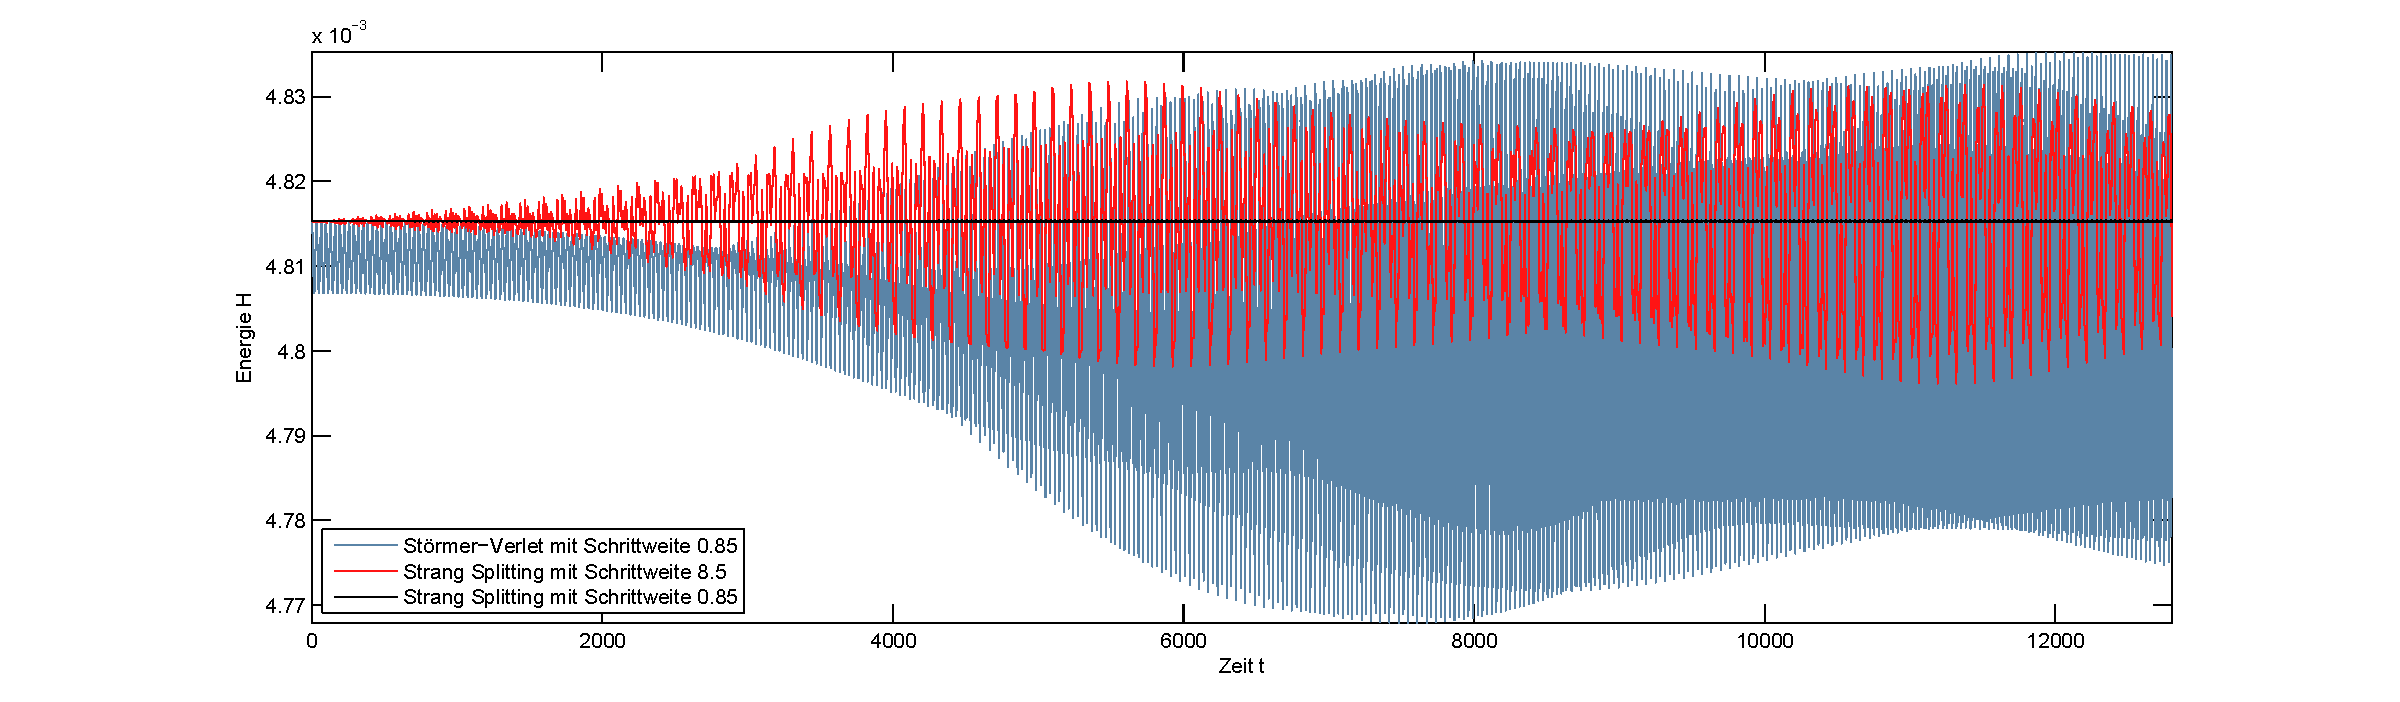
\includegraphics[width=32cm, clip=true, trim=3.3cm 1.2cm 2.2cm 0.5cm, keepaspectratio=true]{implementierung/nr1.pdf}
	    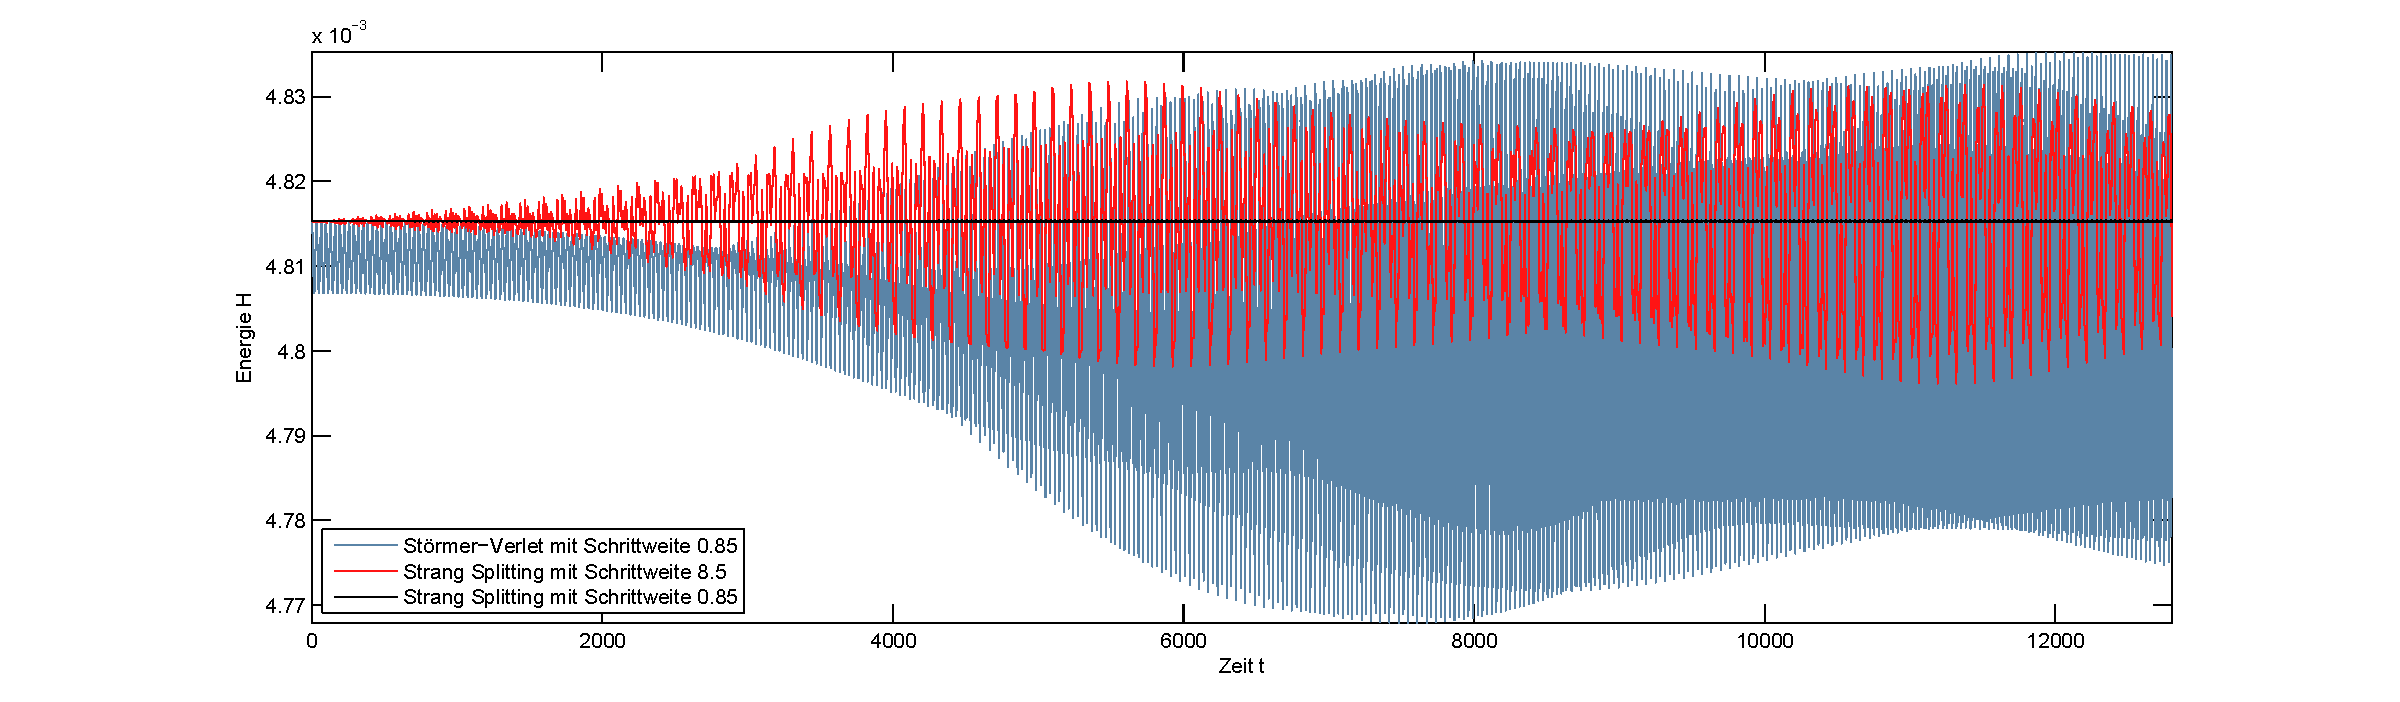
\includegraphics[width=34cm, clip=true, trim=4.0cm 0.4cm 3.8cm 0.3cm, keepaspectratio=true]{implementierung/nr1.pdf}
	  \end{center}
      \vskip2ex
      \textbf{Bemerkung:} Ein Nachteil ist, dass Splitting-Verfahren bei gewissen resonanten Schrittweiten die Energie stark verfälschen können. Das Problem kann teilweise umgangen werden, wenn man die Splitting-Verfahren mit geeigneten impliziten Integratoren kombiniert. Die zweite Grafik zeigt eine solche Situation bei dem vorgestellten Problem. Störmer-Verlet kann übrigens ebenfalls Resonanzprobleme aufweisen, hier dient die blaue Kurve aus der oberen Grafik lediglich als Vergleich. % Die Schrittweite wurde verkleinert, aber die Energie bricht aus.
      %aber das Verfahren liefert trotzdem ein schlechteres Ergebnis.
    \begin{center}
%	    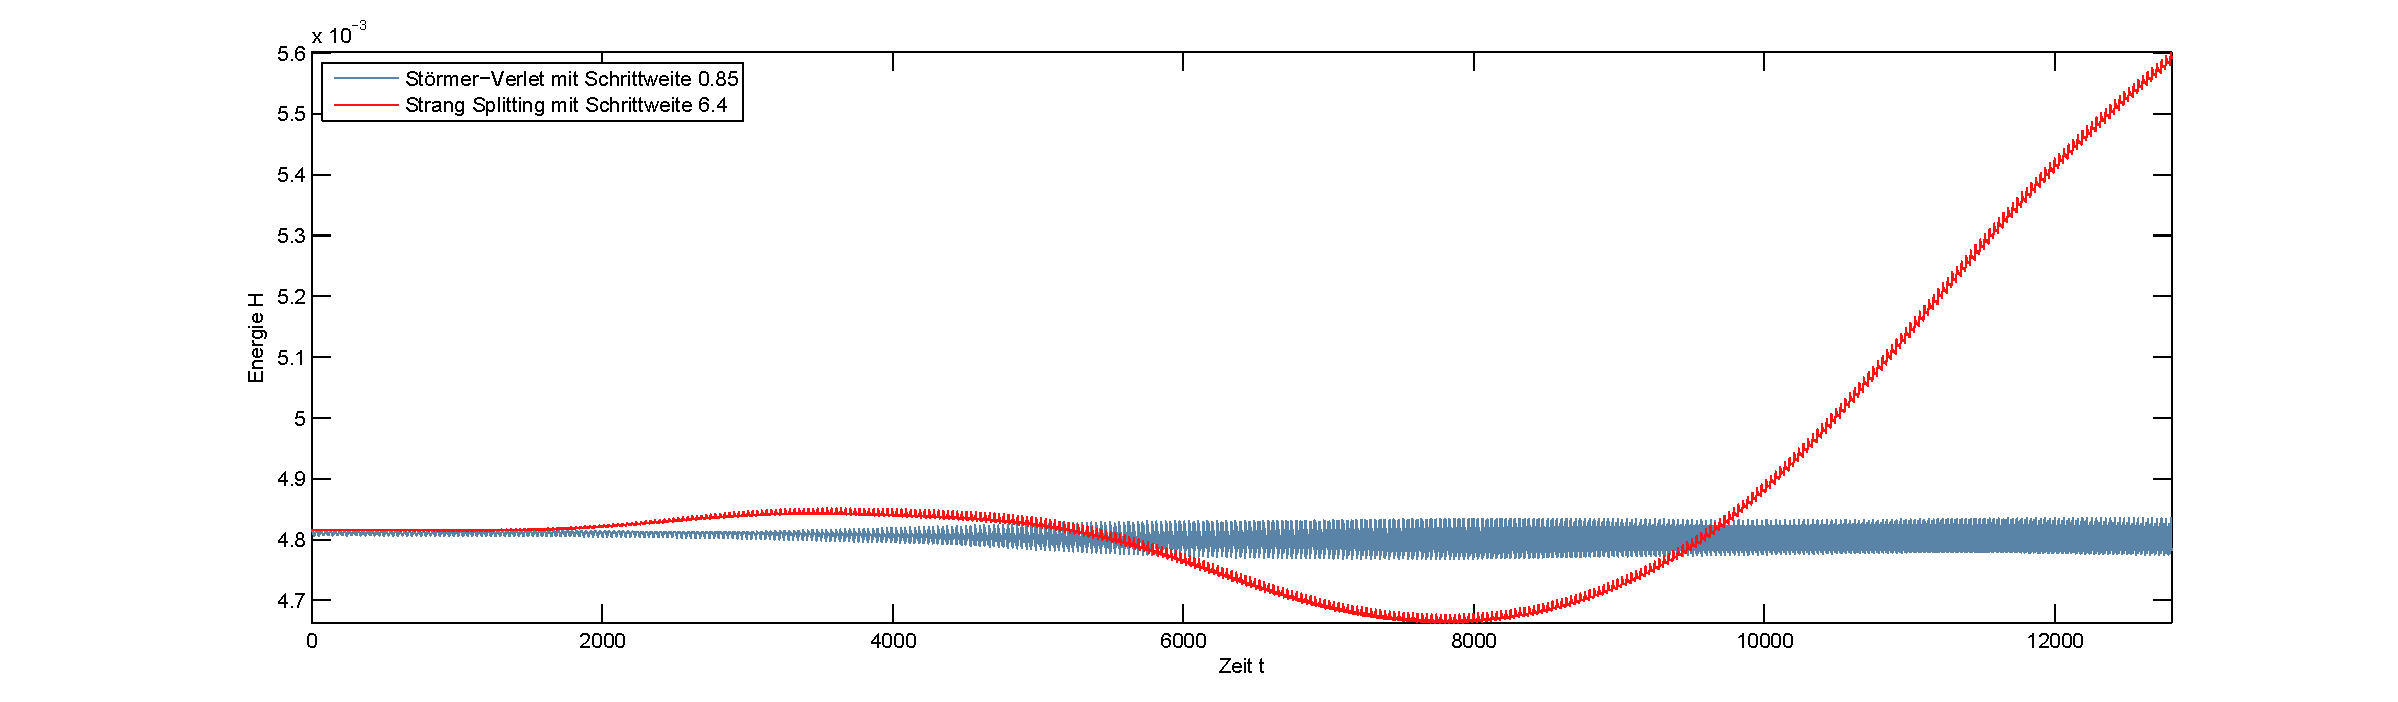
\includegraphics[width=32cm, clip=true, trim=2.7cm 0.85cm 2.1cm 0.2cm, keepaspectratio=true]{implementierung/nr2.pdf}
	    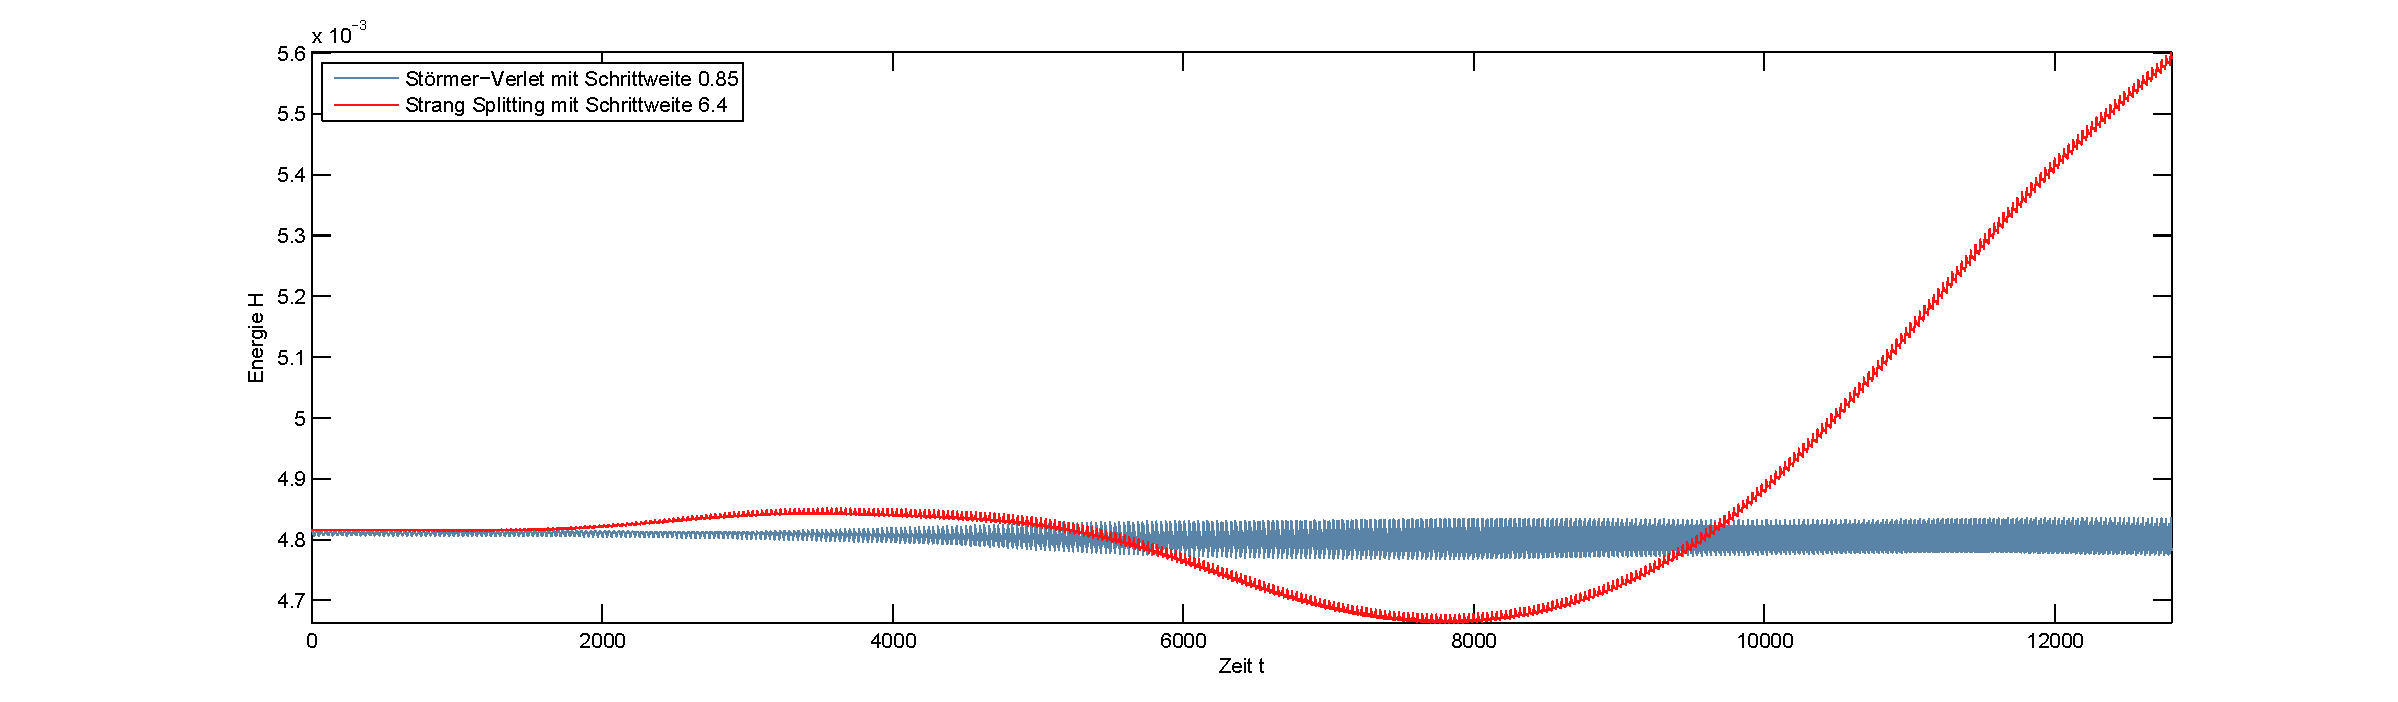
\includegraphics[width=34cm, clip=true, trim=4.1cm 0.4cm 3.8cm 0.3cm, keepaspectratio=true]{implementierung/nr2.pdf}
	  \end{center}
      \vskip2ex
        }
      \end{alertblock}
      \vskip2ex
      \begin{block}{Literatur}
        \rmfamily{
        \begin{flushleft}
        $[1]$ E. Hairer, C. Lubich, G. Wanner: \emph{Geometric Numerical Integration}\\
        $[2]$ B. Leimkuhler, S. Reich: \emph{Simulating Hamiltonian Dynamics}\\
        $[3]$ E. Faou: \emph{Geometric numerical integration of semilinear Hamiltonian PDEs} (http://www.irisa.fr/ipso/perso/faou/ETH/ETH.html)
        \end{flushleft}
        }
      \end{block}

%   \begin{center}
%	    
\includegraphics[width=5in]{logo.pdf}
%	  \end{center}
      \vskip2.5ex
        \begin{flushright}
          \rmfamily{\small Projekt Geometrisch-Numerische Integration, Frühjahrssemester 2010}
        \end{flushright}
    \end{column}
 \end{columns}
\end{frame}
\end{document}
